\documentclass[12pt]{article}

\usepackage{listings}
\usepackage{color}
\usepackage{python}
\usepackage[toc,page]{appendix}
\usepackage{graphicx}
\usepackage[margin=0.5in]{geometry}

\definecolor{dkgreen}{rgb}{0,0.6,0}
\definecolor{gray}{rgb}{0.5,0.5,0.5}
\definecolor{mauve}{rgb}{0.58,0,0.82}

\lstset{frame=tb,
  language=Python,
  aboveskip=3mm,
  belowskip=3mm,
  showstringspaces=false,
  columns=flexible,
  basicstyle={\small\ttfamily},
  numbers=none,
  numberstyle=\tiny\color{gray},
  keywordstyle=\color{blue},
  commentstyle=\color{dkgreen},
  stringstyle=\color{mauve},
  breaklines=false,
  breakatwhitespace=true,
  tabsize=3
}

\title{Characterizing A Geolocation Dataset}
\author{Alexis Barrett \\
	CDS 486 Student}



\begin{document}

\maketitle

\section{Problem Statement}

Given a .csv file of geolocation points of a short leg of a cross-country roadtrip, clean and characterize the dataset. The data file includes time stamped longitude, latitude, altitude, speed and accuracy data points.  Cleaning the dataset will involve logical definition of outliers, and characterization of the dataset will mean plotting the data onto a map and calculating distance traveled. 

\section{Data Exploration}

As seen in the table in Figure \ref{summary1}, the maximum speed is 161.70 kilometers per hour. The minimum speed is 0.0 kilometers per hour.

\begin{figure}[h]
	\centering
	\caption{Table of summary statistics for raw data in file1.csv}
	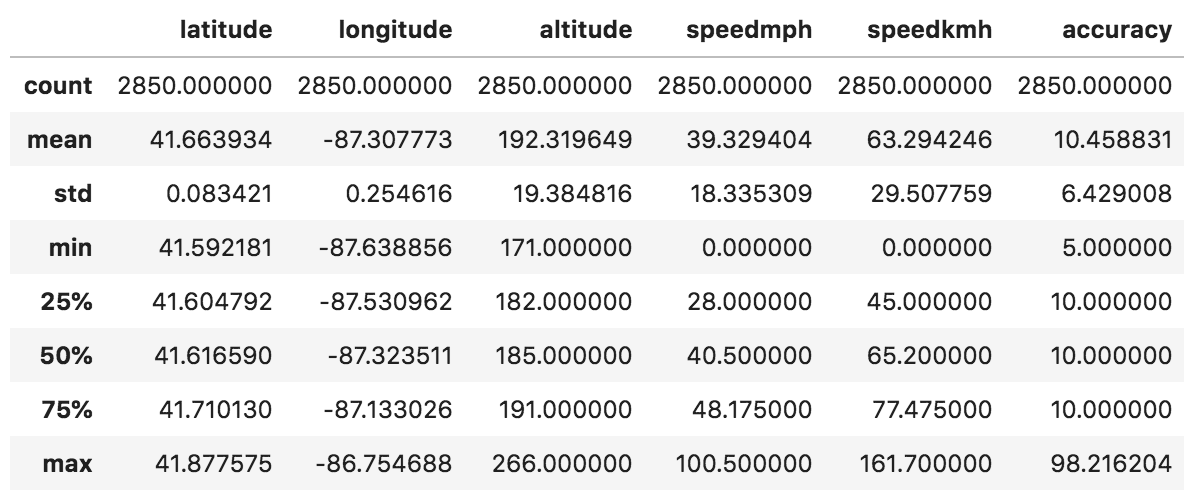
\includegraphics[scale= 0.9]{file1_summary.png}
	\label{summary1}
\end{figure}

\subsection{Accuracy vs. Speed}

  There is a positive correlation between speed and accuracy of the geolocation data, wherein high speeds lead to a large accuracy value. (which in laymen terms means that it is low accuracy, because of the way that accuracy is defined in this dataset.)

\begin{figure}[h]
	\centering
	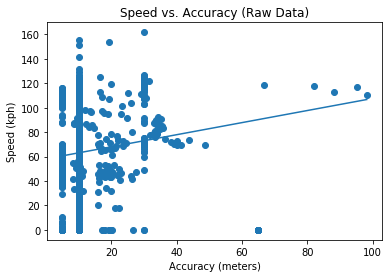
\includegraphics[scale= 0.9]{speed_vs_accuracy_raw.png}
	\caption{Scatterplot of speed vs. accuracy with a linear line of best fit}
	\label{summary1}
\end{figure}

\subsection{Speed Data}

It is unusal for a histogram to be multimodal, as is this histogram, with four distinct peaks. In the case of this dataset however, it can be explained by speed limits. 

\begin{figure}[h]
	\centering
	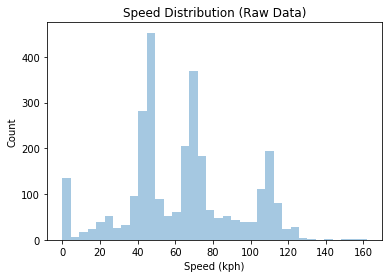
\includegraphics[scale= 1.0]{speed_hist_raw.png}
	\caption{Speed histogram of raw data}
	\label{mg:screenshot}
\end{figure}

\subsection{Outliers}

The lowerbound of the dataset should remain at 0 kph because as automobile travel data, it is reasonable that the car should stop moving, therefore making these data important. The upper bound should be mu + 2 sigma because this value (122.2 kph or about 76 mph) coordinates closely to the speed limit in both Indiana and Illinois of 70 mph. There is also evidence that the accuracy of the data is lower at higher speeds, making this bound more important than a lower bound. It is unlikely that the driver would drive more than 6 mph above the speed limit given the value of the uppermost modes at approximately 110 kph or 68 mph. 

\subsection{Accuracy data}

It would be a good choice to eliminate values above 10 m accuracy from the dataset 
because over 2500 points would be included in the dataset of 2850 points. Proportionally,
this means keeping about 90\% of the data.


\begin{figure}
	\centering
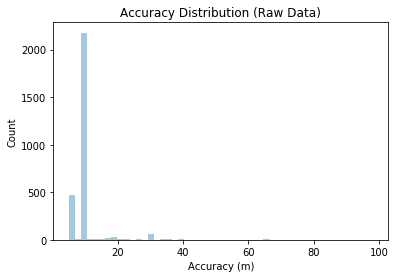
\includegraphics[scale= 1.0]{accuracy_hist.png}
\caption{Accuracy histogram of raw data}
\label{mg:screenshot}
\end{figure}

\section{Data Cleaning}

Outliers will be considered speeds greater than 2 standard deviations above average speed as well as accuracy greater than 10 meters. This definition of outliers will include 214 data points which will be eliminated from the dataset. None were modified. 

\subsection{Analysis of Data Cleaning}

\begin{figure}
	\centering
		\caption{Table of summary statistics for clean data}
	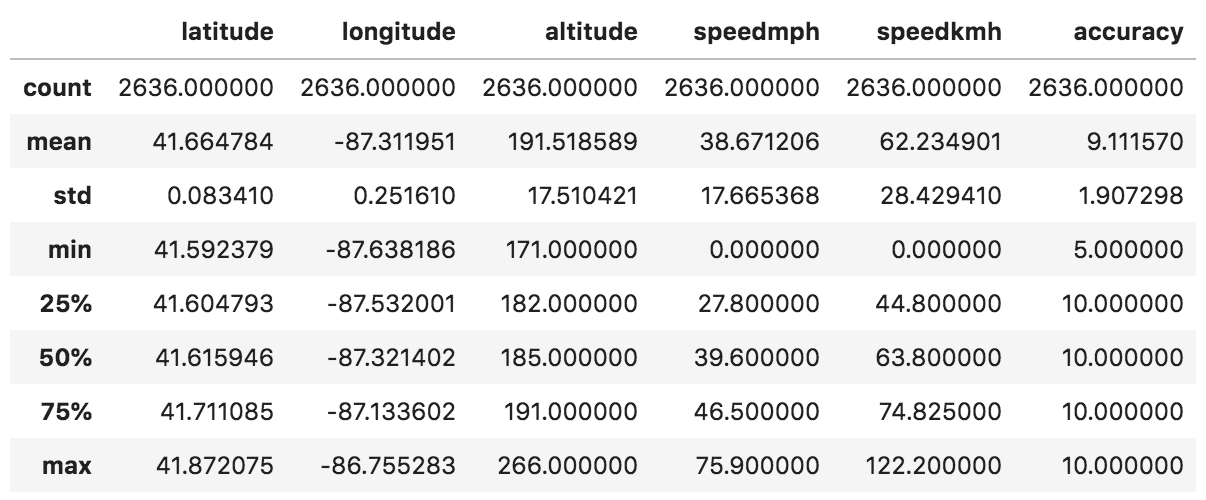
\includegraphics[scale= 0.8]{file1_clean_summary.png}
	\label{file1_clean_summary}
\end{figure}

Comparing the raw data and the cleaned dataset, there are 214 few points in the cleaned dataset. The minimum speed is the same for both dataset, but the maximum speed has been decreased in the cleaned dataset. Accordingly this led to a lowering of the mean value in the cleaned dataset. 

\begin{figure}
	\centering
	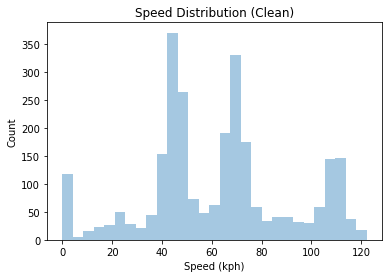
\includegraphics[scale= 0.8]{speed_hist_clean.png}
	\caption{Speed histogram from cleaned dataset.}
	\label{speed_hist_clean}
\end{figure}


The speed distribution as shown in Figure \ref{speed_hist_clean} is quite similar in shape to the speed histogram of the raw dataset. The distribution still is multimodal with four distinct peaks which correlate to stopped, 35 mph speed limit, 55 mph speed limit, and 70 mph speed limit. The most defined difference is in the spread, as values above 125 kph have been eliminated in the cleaned dataset. 

\begin{figure}
	\centering
	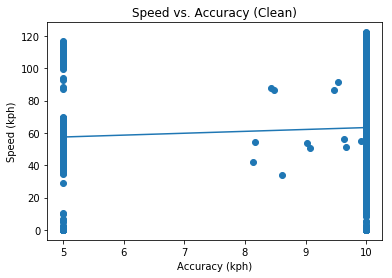
\includegraphics[scale= 0.8]{speed_vs_accuracy_clean.png}
	\caption{Scatterplot of Speed vs. Accuracy from cleaned dataset.}
	\label{speed_vs_accuracy_clean}
\end{figure}

The new plot ranges in the Speed vs. Accuracy plot of cleaned data (see Figure \ref{speed_vs_accuracy_clean}) are refined compared to the raw dataset. Speed is limited to 0 kph to 120 kph, as opposed to the original 0 kph to 165 kph; accuracy is limited to 5 m to 10 m, as opposed to 5 m to 100 m. There is clumping present at 5 m and 10 m accuracy, though there is no longer any correlation in this plot between speed and accuracy. This is ideal because we want speed and accuracy to act as independent variables. 

\begin{figure}
	\centering
		\caption{Table of summary statistics for data cleaned by accuracy = 5 m.}
	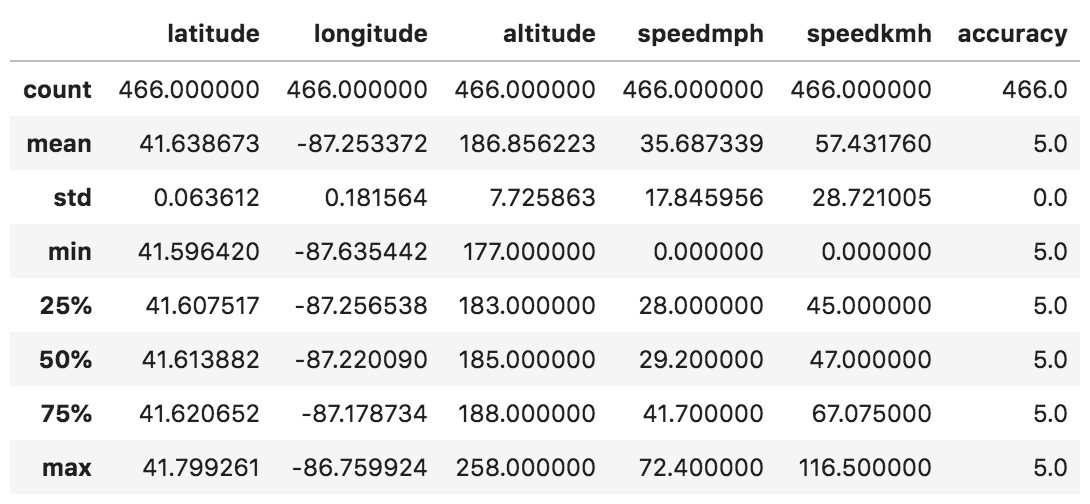
\includegraphics[scale= 0.8]{acc5_summary.png}
	\label{acc5_summary}
\end{figure}

\begin{figure}
	\centering
	\caption{Table of summary statistics for data cleaned by accuracy = 10 m.}
	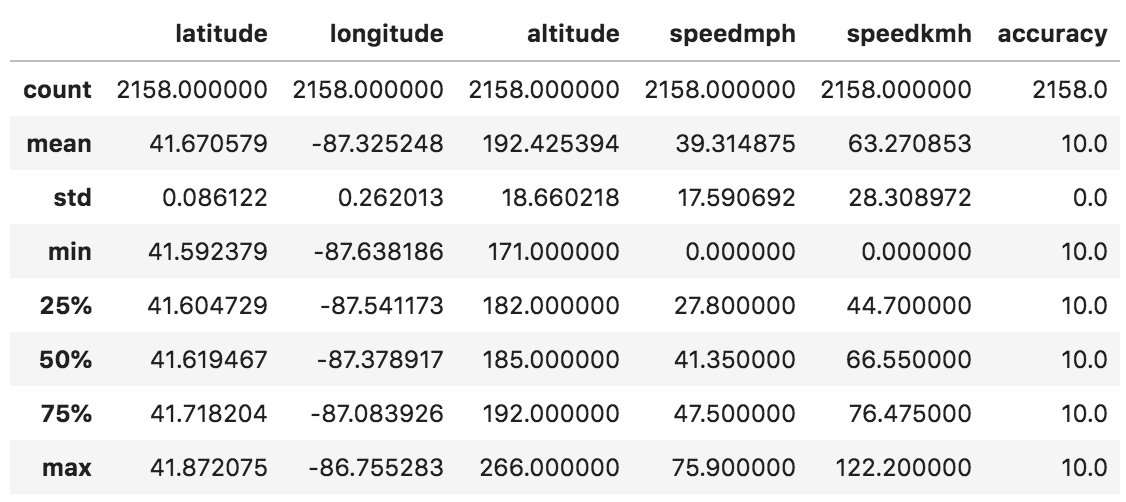
\includegraphics[scale= 0.8]{acc10_summary.png}
	\label{acc10_summary}
\end{figure}

\section{Geopandas}

The map in Figure \ref{map} was generated using shapefiles and the geopandas package. 

\begin{figure}
	\centering
	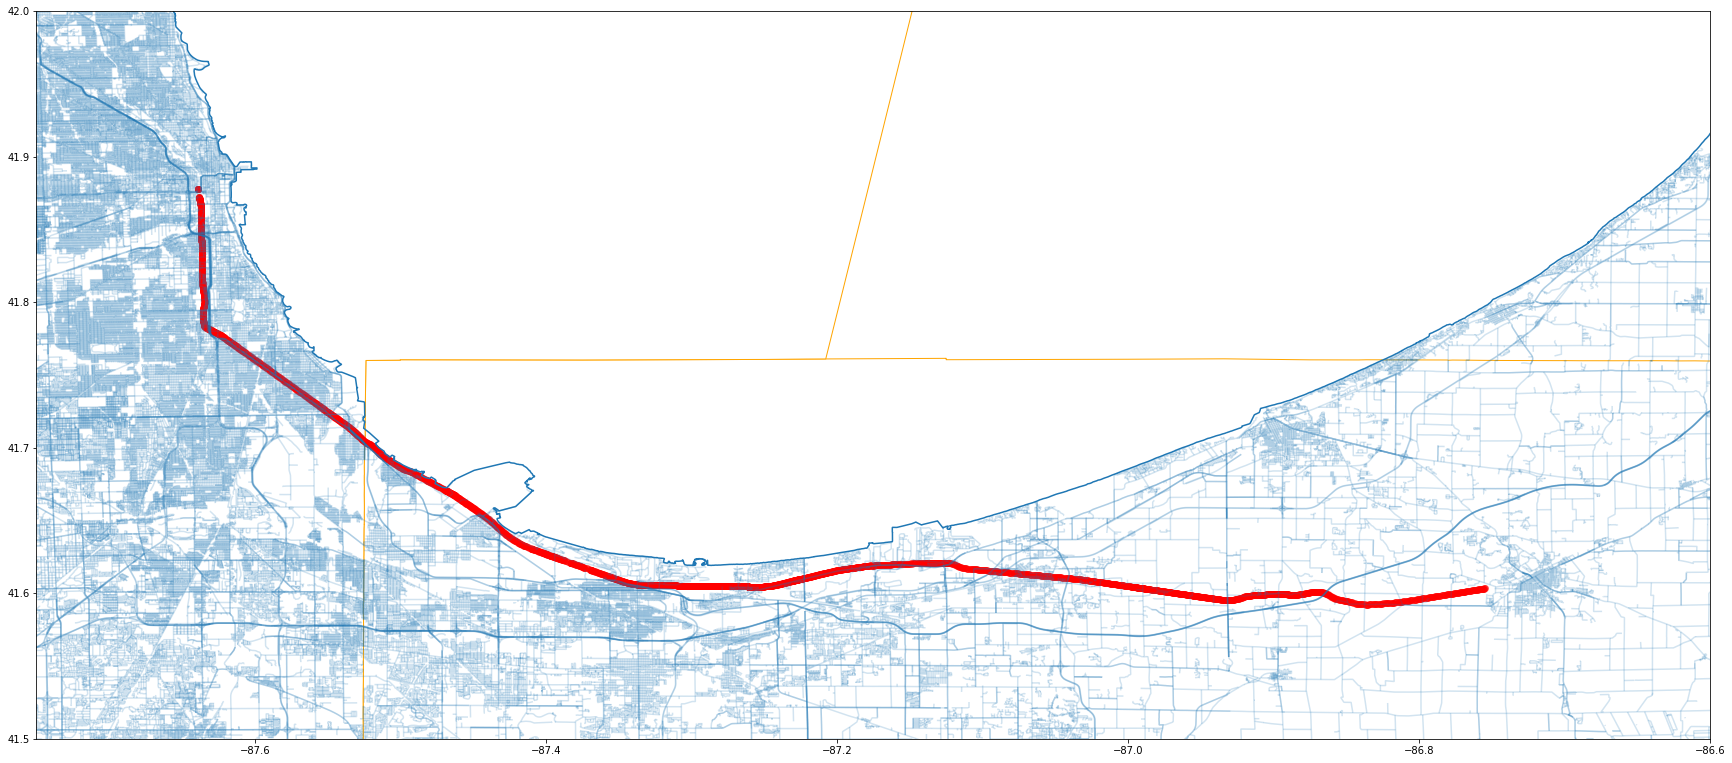
\includegraphics[scale= 0.3]{geo_map.png}
		\caption{Geopandas plot of geolocation data}
	\label{map}
\end{figure}

\subsection{Distance Calculations}

The total distance traveled on this journey as recorded by the geolocation data is 92.868 km. As the crow flies, distance traveled was 80.76 km.

\section{Teaming Assignment}

\newpage
\section{Appendix}
	\begin{lstlisting}

# coding: utf-8

# In[1]:


import numpy as np
import pandas as pd
import geopandas as gpd
from shapely.geometry import Point
import matplotlib.pyplot as plt
import seaborn as sns
import math

file1 = pd.read_csv('file1.csv', ',')

file1.describe()


# In[2]:


plt.scatter(file1['accuracy'],file1['speedkmh'])
plt.xlabel('Accuracy (meters)')
plt.ylabel('Speed (kph)')
plt.title('Speed vs. Accuracy (Raw Data)')

plt.plot(np.unique(file1['accuracy']),          np.poly1d(np.polyfit(file1['accuracy'], file1['speedkmh'], 1))         (np.unique(file1['accuracy'])))
#There is a positive correlation between speed and accuracy.


# In[3]:


sns.distplot(file1['speedkmh'], kde = False)
plt.title('Speed Distribution (Raw Data)')
plt.ylabel('Count')
plt.xlabel('Speed (kph)')


# In[4]:


mean_speedkmh = file1['speedkmh'].mean()
#The average speed for this dataset is 63.29 kph.

std_speedkmh = file1['speedkmh'].std()
#29.5 kph
upperbound_2sig = mean_speedkmh + 2 * std_speedkmh
#122.3 kph ~ 76 mph
upperbound_3sig = mean_speedkmh + 3 * std_speedkmh
#151.8 kph ~ 94 mph


# In[5]:


sns.distplot(file1['accuracy'], kde = False)
plt.title('Accuracy Distribution (Raw Data)')
plt.xlabel('Accuracy (m)')
plt.ylabel('Count')


# In[6]:


file1_clean = file1.loc[(file1['speedkmh'] < upperbound_2sig) &                         (file1['accuracy'] <= 10)]

file1_clean.describe()


# In[7]:


sns.distplot(file1_clean['speedkmh'], kde = False)
plt.title('Speed Distribution (Clean)')
plt.xlabel('Speed (kph)')
plt.ylabel('Count')


# In[8]:


plt.scatter(file1_clean['accuracy'],file1_clean['speedkmh'])

plt.plot(np.unique(file1_clean['accuracy']),          np.poly1d(np.polyfit(file1_clean['accuracy'], file1_clean['speedkmh'], 1))         (np.unique(file1_clean['accuracy'])))

plt.title('Speed vs. Accuracy (Clean)')
plt.xlabel('Accuracy (kph)')
plt.ylabel('Speed (kph)')


#There is clumping present at 5 m and 10 m accuracy, though there is no longer any 
#correlation in this plot between speed and accuracy. This is ideal because we want 
#speed and accuracy to act as independent variables. 


# In[9]:


file1_clean_acc10 = file1_clean.loc[(file1['accuracy'] == 10.0)]
file1_clean_acc5 = file1_clean.loc[(file1['accuracy'] == 5.0)]

file1_clean_acc10.describe()


# In[10]:


file1_clean_acc5.describe()


# In[12]:


file1_clean['Coordinates'] = list(zip(file1_clean.longitude, file1_clean.latitude))

file1_clean['Coordinates'] = file1_clean['Coordinates'].apply(Point)

geofile1 = gpd.GeoDataFrame(file1_clean, geometry='Coordinates')

usa = gpd.read_file('tl_2018_us_state/tl_2018_us_state.shp')
coastline = gpd.read_file('tl_2018_us_coastline/tl_2018_us_coastline.shp')
laporte_in = gpd.read_file('tl_2018_18091_roads/tl_2018_18091_roads.shp')
lake_in = gpd.read_file('tl_2018_18089_roads/tl_2018_18089_roads.shp')
porter_in = gpd.read_file('tl_2018_18127_roads/tl_2018_18127_roads.shp')
cook_il = gpd.read_file('tl_2018_17031_roads/tl_2018_17031_roads.shp')
berrian_mi = gpd.read_file('tl_2018_26021_roads/tl_2018_26021_roads.shp')

#https://www.census.gov/cgi-bin/geo/shapefiles/index.php?

fig, ax = plt.subplots(figsize = (30,30))
ax.set_xlim([-87.75, -86.6])
ax.set_ylim([41.5, 42.0])

usa[usa.NAME == 'Indiana'].plot(ax = ax, color='white', edgecolor='orange')
usa[usa.NAME == 'Illinois'].plot(ax = ax, color='white', edgecolor='orange')
laporte_in.plot(ax = ax, alpha = 0.2)
lake_in.plot(ax = ax, alpha = 0.2)
porter_in.plot(ax = ax, alpha = 0.2)
cook_il.plot(ax = ax, alpha = 0.2)
berrian_mi.plot(ax = ax, alpha = 0.2)
coastline.plot(ax = ax)

#Chicago, IL to La Porte, IN

geofile1.plot(ax=ax, color='red', alpha = 0.5)

plt.title('Geolocation Map of Illinois and Indiana Leg of Cross-Country Roadtrip', fontsize=20)
plt.xlabel('Longitude', fontsize=16)
plt.ylabel('Latitude', fontsize=16)
plt.show()


# In[13]:


#https://www.thoughtco.com/degree-of-latitude-and-longitude-distance-4070616
#Latitude: 1 deg = 111 km
#Longitude: 1 deg = 85 km

start = (-86.75528299999999, 41.603271)
end = (-87.638186, 41.872075)

delta_long = start[0] - end[0]
delta_lat = start[1] - end[1]

delta_km_ew = delta_long * 85
delta_km_ns = delta_lat * 111

distance = (delta_km_ew**2 + delta_km_ns**2)**0.5

print(distance)


# In[14]:


total_distance = 0
for x in range(2635):
start = (file1_clean.iloc[x,2], file1_clean.iloc[x,1])
end = (file1_clean.iloc[x+1,2], file1_clean.iloc[x+1,1])

delta_long = start[0] - end[0]
delta_lat = start[1] - end[1]

delta_km_ew = delta_long * 85
delta_km_ns = delta_lat * 111

distance = (delta_km_ew**2 + delta_km_ns**2)**0.5

total_distance = total_distance + distance
print(total_distance)



		
		
	\end{lstlisting}


\end{document}